
\newpage
\section{Naive GPU Implementation}
\begin{figure}[h]
    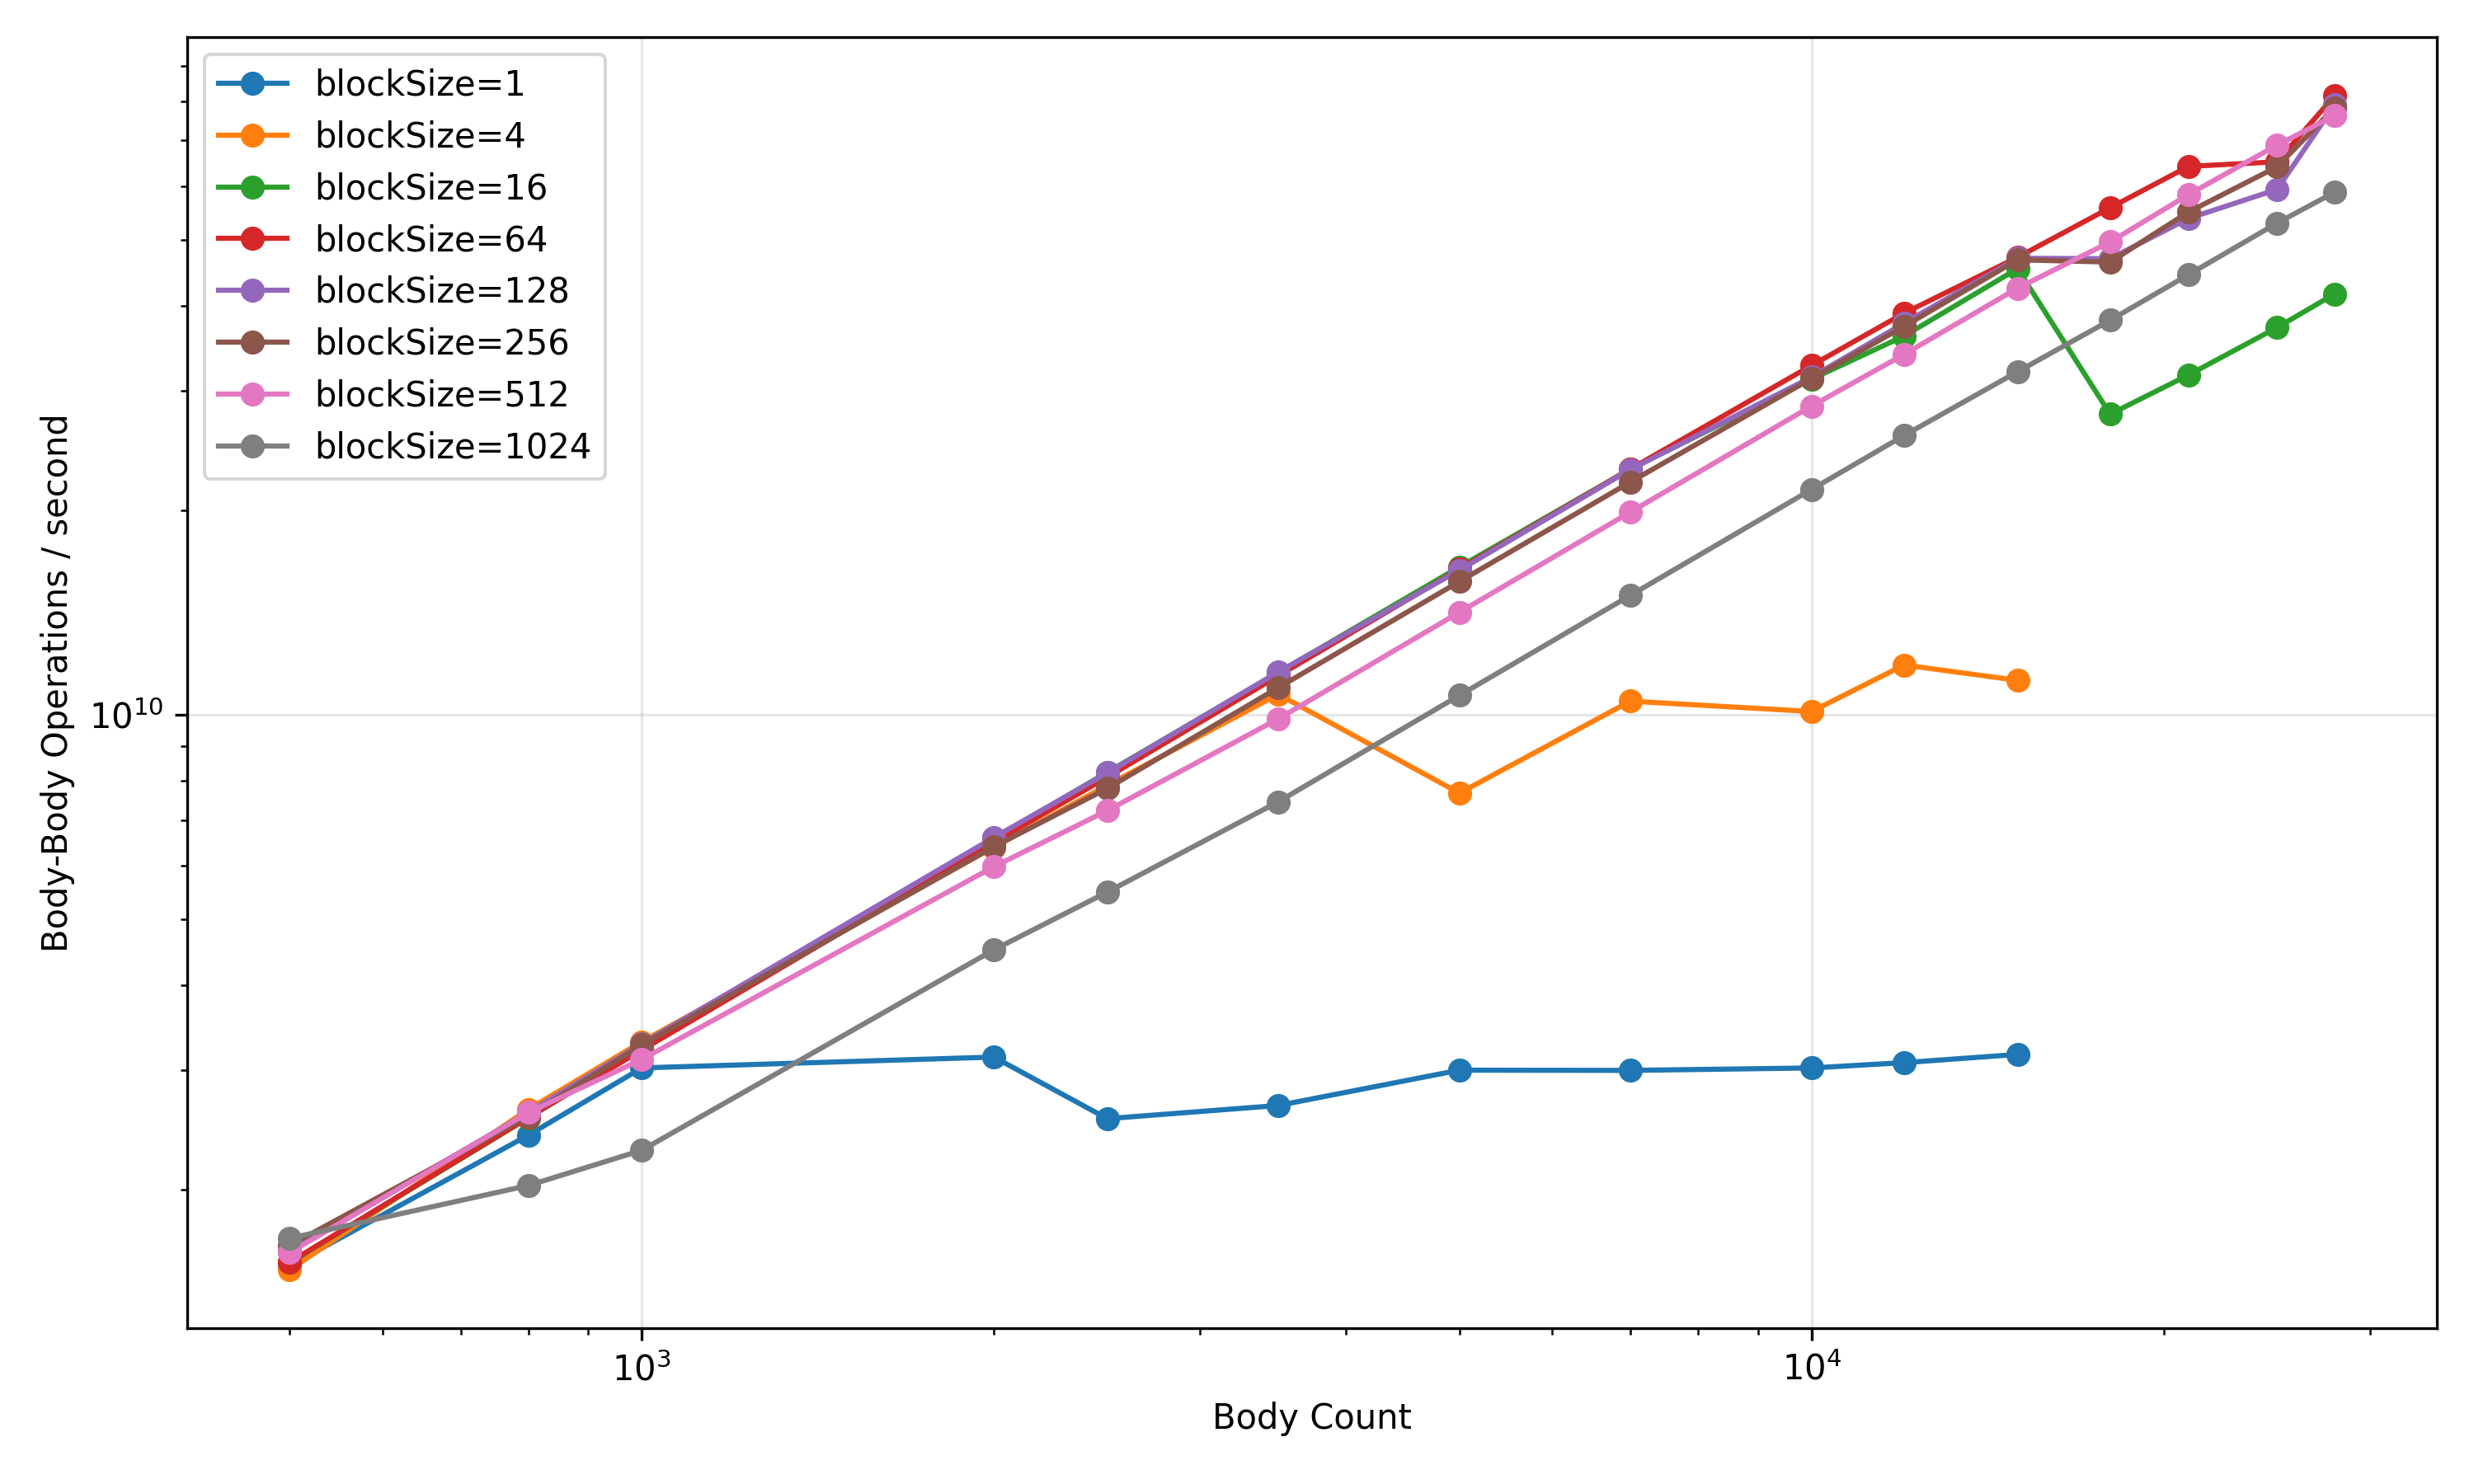
\includegraphics[width=1.0\textwidth]{../noah/plots/7_1.png}
    \caption{Naive GPU Performance (500 iterations)}
    \label{fig:1}
\end{figure}

Plot \ref{fig:1} shows the performance of the naive GPU implementation over 500 iterations. The measurements where taken as median values to account for outliers.\\
Performance increases with larger block sizes, as more warps can be scheduled concurrently. For block sizes of 256 and higher, performance is quite similar, as the GPU cores are well utilized. For smaller block sizes, performance drops significantly for larger matrices, since the CUDA cores are underutilized.\\
This means that the overall performance (interactions per second) also increases with a larger problem size, up to the point where a limit for the current block size is reached. From there, performance stays roughly constant.\\
We can also see that the larger block sizes (512 and 1024) perform slightly worse than 64-256 range, which might be due to a reduced flexibility of scheduling.